\documentclass[aspectratio=169,10pt]{beamer}

\usepackage[T1]{fontenc}
\usepackage[utf8]{inputenc}
\usepackage{lmodern}
\usepackage{amsmath}
\usepackage{booktabs}
\usepackage{array}
\usepackage[round,authoryear]{natbib}
\usepackage{tikz}
\usepackage{pgfplots}
\usepackage{pgfplotstable}
\usepackage{appendixnumberbeamer}
\usetikzlibrary{arrows.meta,backgrounds,calc,fit,positioning,shapes.geometric}
\usepgfplotslibrary{groupplots}
\pgfplotsset{compat=1.18}

\definecolor{SymNavy}{HTML}{12314A}
\definecolor{SymTeal}{HTML}{1E6F78}
\definecolor{SymGold}{HTML}{D89B2B}
\definecolor{SymSand}{HTML}{F5F1E8}
\definecolor{SymSlate}{HTML}{53636F}
\definecolor{SymInk}{HTML}{1F2328}
\definecolor{SymSoftRed}{HTML}{B75D4A}
\definecolor{SymSoftGreen}{HTML}{4F7A4A}
\definecolor{SymSoftBlue}{HTML}{5B82B8}
\definecolor{SymSoftGray}{HTML}{B9C1C7}

\setbeamercolor{background canvas}{bg=SymSand}
\setbeamercolor{normal text}{fg=SymInk,bg=SymSand}
\setbeamercolor{frametitle}{fg=SymNavy}
\setbeamercolor{title}{fg=white,bg=SymNavy}
\setbeamercolor{subtitle}{fg=SymSand}
\setbeamercolor{structure}{fg=SymTeal}
\setbeamercolor{alerted text}{fg=SymSoftRed}
\setbeamercolor{block title}{fg=white,bg=SymTeal}
\setbeamercolor{block body}{fg=SymInk,bg=white}
\setbeamercolor{footline}{fg=SymSand,bg=SymNavy}

\setbeamertemplate{navigation symbols}{}
\setbeamertemplate{itemize item}{\color{SymGold}$\blacktriangleright$}
\setbeamertemplate{itemize subitem}{\color{SymTeal}$\circ$}
\setbeamertemplate{frametitle}{
  \vspace{0.2em}
  \insertframetitle\par
  \vspace{0.25em}
  {\color{SymGold}\rule{\linewidth}{1pt}}
}
\setbeamertemplate{footline}{
  \leavevmode
  \hbox{
    \begin{beamercolorbox}[wd=.8\paperwidth,ht=2.8ex,dp=1.2ex,leftskip=1em]{footline}
      \insertshorttitle
    \end{beamercolorbox}
    \begin{beamercolorbox}[wd=.2\paperwidth,ht=2.8ex,dp=1.2ex,rightskip=1em]{footline}
      \hfill\insertframenumber/\inserttotalframenumber
    \end{beamercolorbox}
  }
}

\newcommand{\decktitle}[2]{
  \begin{frame}[plain]
    \begin{tikzpicture}[remember picture,overlay]
      \fill[SymNavy] (current page.south west) rectangle (current page.north east);
      \fill[SymTeal] ([xshift=-0.5cm,yshift=-2.3cm]current page.north east)
        rectangle ([xshift=0cm,yshift=0cm]current page.north east);
      \fill[SymGold] ([xshift=0cm,yshift=0cm]current page.south west)
        rectangle ([xshift=\paperwidth,yshift=0.28cm]current page.south west);
    \end{tikzpicture}
    \vspace{1.8cm}
    {\usebeamerfont{title}\color{white}\LARGE #1\par}
    \vspace{0.4cm}
    {\usebeamerfont{subtitle}\color{SymSand}\large #2\par}
    \vfill
    {\color{SymSand}\small Companion source for \texttt{docs/symkan\_manuscript.md}\par}
    \vspace{0.3cm}
  \end{frame}
}

\newcommand{\evidence}[1]{
  \vfill
  {\color{SymSlate}\tiny\textbf{Evidence boundary:} #1\par}
}

\newcommand{\takeaway}[1]{
  \begin{block}{Takeaway}
    #1
  \end{block}
}

\newcommand{\metricbox}[3]{
  \begin{tikzpicture}
    \node[
      rounded corners=4pt,
      draw=SymSoftGray,
      fill=white,
      minimum width=\linewidth,
      inner sep=8pt
    ] {
      \begin{minipage}{0.92\linewidth}
        {\footnotesize\color{SymSlate}#1\par}
        {\Large\color{SymNavy}\textbf{#2}\par}
        {\scriptsize\color{SymSlate}#3\par}
      \end{minipage}
    };
  \end{tikzpicture}
}

\newcommand{\auditpill}[2]{
  \tikz[baseline=(label.base)]{
    \node[
      rounded corners=5pt,
      fill=#1!18,
      draw=#1!55!black,
      inner xsep=6pt,
      inner ysep=2pt
    ] (label) {\scriptsize\textbf{#2}};
  }
}

\newcommand{\smallsource}[1]{{\scriptsize\color{SymSlate}#1}}

\newcommand{\literature}[1]{
  {\color{SymSlate}\tiny\textbf{Research context:} #1\par}
}

% Values copied from docs/symkan_manuscript.md.

\pgfplotstableread{
variant acc auc runtime core val
baseline 0.777433 0.956107 153.470521 33.867724 -0.672284
adaptive 0.742533 0.945706 209.552334 47.499191 -0.646339
adaptiveauto 0.751467 0.946249 130.715215 33.259280 -0.552361
}\defaultstrategydata

\pgfplotstableread{
variant acc complexity symtime
full 0.7807 126.90 33.58
wostagewise 0.4430 48.44 16.64
wopruning 0.8017 194.33 43.51
wocompact 0.7577 120.10 41.34
wolayerwiseft 0.7838 126.90 20.41
}\ablationdata

\pgfplotstableread{
variant acc auc val symtime
full 0.7807 0.9548 -0.6135 33.58
layerwiseftesreg 0.7807 0.9548 -0.6135 33.28
wolayerwiseft 0.7838 0.9544 -0.5937 20.41
}\layerwiseftdata

\pgfplotstableread{
variant acc auc runtime core val
baseline 0.777467 0.951264 69.864499 33.297856 -0.486988
baselineicbr 0.788667 0.961440 62.462939 19.013927 -0.409281
}\layeredcomparedata

\pgfplotstableread{
variant acc auc runtime core val
baselinefastlib 0.794000 0.962537 112.233492 75.187859 -0.451777
baselineicbrfastlib 0.793233 0.962634 69.944645 31.990798 -0.456489
}\fastlibcomparedata

\def\LayeredSpeedup{1.751763}
\def\FastlibSpeedup{2.350452}
\def\FullLibAcc{0.795433}
\def\FullLibAuc{0.963225}
\def\FullLibCore{35.218785}
\def\FullLibRuntime{41.757397}
\def\FullLibTargetRtwo{0.601003}


\title[SymKAN companion deck]{SymKAN companion deck}
\author{Repository-aligned Beamer source}
\date{2026-04-06}

\begin{document}

\decktitle{SymKAN as an auditable post-training symbolization workflow}{Companion slides for manuscript-aligned defense or paper talk}

\begin{frame}{Thesis and writing boundary}
  \begin{columns}[T,onlytextwidth]
    \column{0.54\textwidth}
      \begin{block}{What the deck argues}
        \begin{itemize}
          \item SymKAN is a controlled workflow around a trained KAN, not a new trainer.
          \item The scientific object is the pipeline: readiness, symbolic preparation, backend completion, validation, and archival.
          \item The central contribution is methodological discipline: reproducible, comparable, auditable evidence.
        \end{itemize}
      \end{block}
    \column{0.43\textwidth}
      \begin{block}{What the deck does not claim}
        \begin{itemize}
          \item Not a general symbolic regression system.
          \item Not a proof of broader neural-symbolic superiority.
          \item Not a large-sample significance study.
        \end{itemize}
      \end{block}
      \takeaway{Keep every oral claim inside the manuscript's evidence family and dated rerun boundary.}
  \end{columns}
  \literature{KAN framing follows \citep{liu2024kan}; the post-hoc symbolic-modeling context follows \citep{cranmer2020symbolicmodels}; symbolic-regression background follows \citep{udrescu2020aifeynman,petersen2019deepsr,lacava2021contemporarysr}.}
  \evidence{Manuscript abstract, Sections 1, 2, and 9.}
\end{frame}

\begin{frame}{Pipeline decomposition}
  \centering
  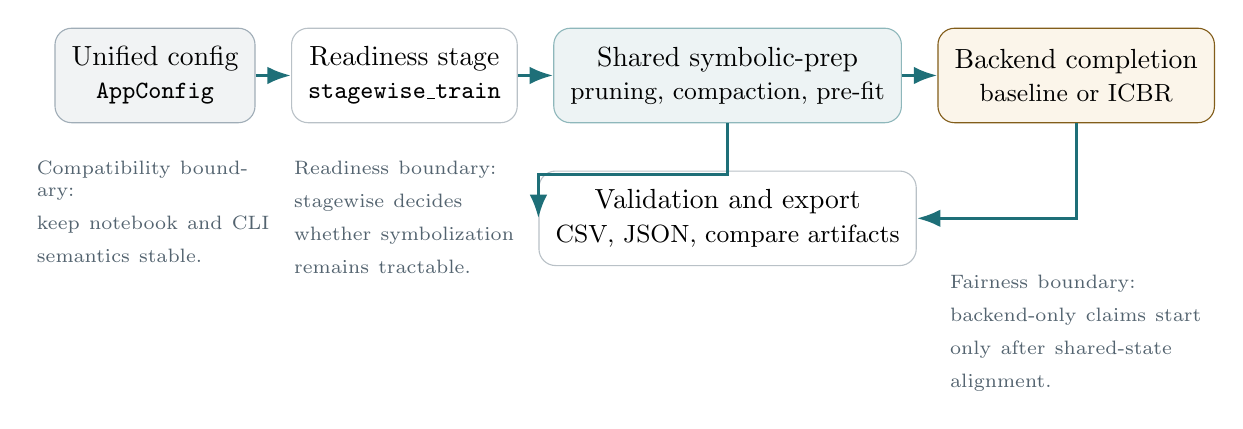
\begin{tikzpicture}[
      node distance=0.6cm and 0.45cm,
      box/.style={
        rounded corners=6pt,
        draw=SymSoftGray,
        fill=white,
        minimum height=1.2cm,
        minimum width=2.35cm,
        align=center,
        inner sep=6pt
      },
      arrow/.style={-{Latex[length=3mm]}, very thick, draw=SymTeal}
    ]
    \node[box, fill=SymNavy!6, draw=SymNavy!40] (config) {Unified config\\\small \texttt{AppConfig}};
    \node[box, right=of config] (stagewise) {Readiness stage\\\small \texttt{stagewise\_train}};
    \node[box, right=of stagewise, fill=SymTeal!8, draw=SymTeal!50] (prep) {Shared symbolic-prep\\\small pruning, compaction, pre-fit};
    \node[box, right=of prep, fill=SymGold!10, draw=SymGold!60!black] (backend) {Backend completion\\\small baseline or ICBR};
    \node[box, below=of prep, minimum width=3.2cm] (validate) {Validation and export\\\small CSV, JSON, compare artifacts};

    \draw[arrow] (config) -- (stagewise);
    \draw[arrow] (stagewise) -- (prep);
    \draw[arrow] (prep) -- (backend);
    \draw[arrow] (backend.south) |- (validate.east);
    \draw[arrow] (prep.south) -- ++(0,-0.65) -| (validate.west);

    \node[below=0.35cm of config, align=left, text width=3.0cm] {\smallsource{Compatibility boundary:\\ keep notebook and CLI semantics stable.}};
    \node[below=0.35cm of stagewise, align=left, text width=2.8cm] {\smallsource{Readiness boundary:\\ stagewise decides whether symbolization remains tractable.}};
    \node[below=1.8cm of backend, align=left, text width=3.2cm] {\smallsource{Fairness boundary:\\ backend-only claims start only after shared-state alignment.}};
  \end{tikzpicture}
  \evidence{Manuscript Sections 2.1, 3.1, 3.2; ARCHITECTURE.md workflow split.}
\end{frame}

\begin{frame}{Evidence hierarchy before results}
  \small
  \begin{tabular}{>{\raggedright\arraybackslash}p{0.28\linewidth} >{\raggedright\arraybackslash}p{0.33\linewidth} >{\raggedright\arraybackslash}p{0.31\linewidth}}
    \toprule
    \textbf{Evidence line} & \textbf{Question answered} & \textbf{Allowed claim} \\
    \midrule
    Engineering rerun (2026-03-18) & Why the default path remains \texttt{baseline} & Current quality-cost anchor for the maintained workflow \\
    Module ablation & What each module is for & Stagewise as readiness, pruning as complexity control, compaction as throughput tradeoff \\
    LayerwiseFT topic report & Whether LayerwiseFT should stay default & Opt-in only; no stable net benefit for the current 2-layer setting \\
    Layered paired compare (2026-04-01) & When backend fairness is strongest & Conservative backend-only evidence with shared-state alignment \\
    FAST\_LIB paired compare & Whether speedup survives library expansion & Speed boundary still holds; quality mostly flat \\
    Full-library one-sided slice & Whether the path still runs & Supplementary viability only; not a fairness proof \\
    \bottomrule
  \end{tabular}
  \vspace{0.4cm}
  \takeaway{Do not compress these lines into one master chart. Each line answers a different methodological question.}
  \literature{The reporting discipline follows broader reproducibility and benchmark concerns in machine learning and scientific ML \citep{pineau2020reproducibility,thiyagalingam2022scimlbenchmarks,kapoor2023leakage}.}
  \evidence{Manuscript Section 4.2 and Section 8.}
\end{frame}

\begin{frame}{Default path: why \texttt{baseline} remains the anchor}
  \begin{columns}[T,onlytextwidth]
    \column{0.64\textwidth}
      \begin{tikzpicture}
        \begin{groupplot}[
          group style={group size=2 by 1, horizontal sep=1.8cm},
          width=0.47\linewidth,
          height=0.47\textheight,
          ybar,
          ymin=0,
          axis lines*=left,
          xtick=data,
          xticklabel style={font=\scriptsize, rotate=18, anchor=east},
          yticklabel style={font=\scriptsize},
          legend style={font=\scriptsize, draw=none, fill=none, at={(0.5,1.16)}, anchor=south, legend columns=2},
          nodes near coords,
          every node near coord/.append style={font=\tiny, rotate=90, anchor=west},
        ]
          \nextgroupplot[
            title={Quality},
            symbolic x coords={baseline,adaptive,adaptiveauto},
            xticklabels={baseline,adaptive,adaptive\_auto},
            ylabel={score},
            ymin=0.70,
            ymax=1.00,
          ]
            \addplot[fill=SymTeal] table[x=variant,y=acc]{\defaultstrategydata};
            \addplot[fill=SymGold] table[x=variant,y=auc]{\defaultstrategydata};
            \legend{final\_acc,macro\_auc}
          \nextgroupplot[
            title={Cost},
            symbolic x coords={baseline,adaptive,adaptiveauto},
            xticklabels={baseline,adaptive,adaptive\_auto},
            ylabel={seconds},
            ymin=0,
            ymax=225,
          ]
            \addplot[fill=SymSoftBlue] table[x=variant,y=runtime]{\defaultstrategydata};
            \addplot[fill=SymSoftRed] table[x=variant,y=core]{\defaultstrategydata};
            \legend{run\_total\_wall\_time\_s,symbolic\_core\_seconds}
        \end{groupplot}
      \end{tikzpicture}
    \column{0.33\textwidth}
      \metricbox{Quality anchor}{baseline}{Highest mean \texttt{final\_acc} and \texttt{macro\_auc} among maintained strategy variants.}
      \vspace{0.3cm}
      \metricbox{Why not \texttt{adaptive\_auto}}{Faster, not primary}{Runtime drops, but the manuscript does not promote it to the quality mainline.}
      \vspace{0.3cm}
      \metricbox{Why not \texttt{adaptive}}{Higher cost, lower quality}{The evidence does not support replacing the default path.}
  \end{columns}
  \evidence{Manuscript Section 5.1; dated engineering rerun family 2026-03-18.}
\end{frame}

\begin{frame}{Ablation: module roles are evidence-driven}
  \begin{columns}[T,onlytextwidth]
    \column{0.64\textwidth}
      \begin{tikzpicture}
        \begin{groupplot}[
          group style={group size=3 by 1, horizontal sep=1.1cm},
          width=0.31\linewidth,
          height=0.44\textheight,
          ybar,
          ymin=0,
          axis lines*=left,
          xtick=data,
          xticklabel style={font=\tiny, rotate=45, anchor=east},
          yticklabel style={font=\scriptsize},
          nodes near coords,
          every node near coord/.append style={font=\tiny, rotate=90, anchor=west},
          symbolic x coords={full,wostagewise,wopruning,wocompact,wolayerwiseft},
        ]
          \nextgroupplot[title={final\_acc}, ylabel={score}, ymax=0.9]
            \addplot[fill=SymTeal] table[x=variant,y=acc]{\ablationdata};
          \nextgroupplot[title={expr complexity}, ylabel={mean}, ymax=210]
            \addplot[fill=SymGold] table[x=variant,y=complexity]{\ablationdata};
          \nextgroupplot[title={symbolic time}, ylabel={seconds}, ymax=50]
            \addplot[fill=SymSoftBlue] table[x=variant,y=symtime]{\ablationdata};
        \end{groupplot}
      \end{tikzpicture}
    \column{0.33\textwidth}
      \begin{block}{Operational reading}
        \begin{itemize}
          \item Removing Stagewise collapses readiness.
          \item Removing pruning can improve quality, but complexity and symbolic cost expand sharply.
          \item Removing compaction improves \texttt{validation\_mean\_r2}, but doubles the effective input dimension.
        \end{itemize}
      \end{block}
      \takeaway{The default workflow is not a stack of helpful tricks. Each module pays for a distinct engineering role.}
  \end{columns}
  \evidence{Manuscript Section 5.2 and the ablation evidence family it names.}
\end{frame}

\begin{frame}{LayerwiseFT stays opt-in}
  \begin{columns}[T,onlytextwidth]
    \column{0.58\textwidth}
      \begin{tikzpicture}
        \begin{axis}[
          width=\linewidth,
          height=0.5\textheight,
          xbar,
          xmin=0,
          xmax=36,
          axis lines*=left,
          y dir=reverse,
          symbolic y coords={full,layerwiseftesreg,wolayerwiseft},
          ytick=data,
          yticklabels={full,layerwiseft\_esreg,wolayerwiseft},
          yticklabel style={font=\scriptsize},
          xlabel={symbolic time (s)},
          nodes near coords,
          every node near coord/.append style={font=\tiny},
        ]
          \addplot[fill=SymSoftRed] table[x=symtime,y=variant]{\layerwiseftdata};
        \end{axis}
      \end{tikzpicture}
    \column{0.39\textwidth}
      \metricbox{Accuracy / AUC}{Essentially unchanged}{\texttt{full} and \texttt{layerwiseft\_esreg} share the same means in the manuscript table.}
      \vspace{0.3cm}
      \metricbox{Observed cost}{Still material}{\texttt{wolayerwiseft} reduces symbolic time to 20.41 s with no stable quality loss.}
      \vspace{0.3cm}
      \takeaway{The safe wording is not “LayerwiseFT is useless”, but “no stable net gain for the current 2-layer default”.}
  \end{columns}
  \evidence{Manuscript Section 5.3 and the dedicated LayerwiseFT report family.}
\end{frame}

\begin{frame}{When a backend compare is fair}
  \begin{columns}[T,onlytextwidth]
    \column{0.46\textwidth}
      \begin{block}{Shared-state audit}
        \begin{itemize}
          \item \auditpill{SymSoftGreen}{shared\_numeric\_aligned = True}
          \item \auditpill{SymSoftGreen}{trace\_aligned = True}
          \item \auditpill{SymSoftGreen}{shared\_symbolic\_prep\_aligned = True}
        \end{itemize}
      \end{block}
      \takeaway{Backend-only claims start only after the shared numeric state, trace rhythm, and symbolic-prep state are aligned.}
    \column{0.50\textwidth}
      \begin{block}{Runtime glossary}
        \begin{itemize}
          \item \texttt{symbolic\_core\_seconds}: backend completion core time; primary speed metric.
          \item \texttt{symbolize\_wall\_time\_s}: broader symbolic wall-clock time with extra overhead.
          \item \texttt{run\_total\_wall\_time\_s}: end-to-end run cost; useful for workflow cost, not for pure backend effect.
        \end{itemize}
      \end{block}
      \smallsource{Keep this slide before any ICBR result slide; otherwise the fairness claim sounds stronger than the evidence.}
  \end{columns}
  \literature{The comparison framing is aligned with reproducibility-first evaluation rather than architecture-first rhetoric \citep{pineau2020reproducibility,kapoor2023leakage}.}
  \evidence{Manuscript Sections 3.2, 4.1, 6.1; layered paired compare requires the shared-check files named there.}
\end{frame}

\begin{frame}{Layered paired compare: strongest fairness evidence}
  \begin{columns}[T,onlytextwidth]
    \column{0.58\textwidth}
      \begin{tikzpicture}
        \begin{axis}[
          width=\linewidth,
          height=0.48\textheight,
          xmin=0.5,
          xmax=2.5,
          ymin=0,
          ymax=36,
          xtick={1,2},
          xticklabels={baseline,baseline\_icbr},
          ylabel={symbolic\_core\_seconds},
          axis lines*=left,
          yticklabel style={font=\scriptsize},
          xticklabel style={font=\scriptsize},
        ]
          \addplot[very thick, color=SymSoftRed, mark=*] coordinates {(1,33.297856) (2,19.013927)};
          \node[anchor=west, font=\scriptsize, text=SymSoftRed] at (axis cs:2.03,19.013927) {core time};
        \end{axis}
      \end{tikzpicture}
    \column{0.39\textwidth}
      \metricbox{Core symbolic speedup}{\LayeredSpeedup x}{\texttt{baseline\_icbr} reduces \texttt{symbolic\_core\_seconds} from 33.30 s to 19.01 s.}
      \vspace{0.3cm}
      \metricbox{Same complexity, better quality}{88.33 edges on both sides}{\texttt{final\_acc}, \texttt{macro\_auc}, and \texttt{validation\_mean\_r2} all improve in the manuscript table.}
      \vspace{0.3cm}
      \takeaway{This slide supports “paired backend gain at matched complexity”, not a universal superiority claim.}
  \end{columns}
  \evidence{Manuscript Section 6.1; dated source family 2026-04-01 layered paired compare.}
\end{frame}

\begin{frame}{FAST\_LIB paired compare: speed boundary under library expansion}
  \begin{columns}[T,onlytextwidth]
    \column{0.58\textwidth}
      \begin{tikzpicture}
        \begin{axis}[
          width=\linewidth,
          height=0.48\textheight,
          xmin=0.5,
          xmax=2.5,
          ymin=0,
          ymax=80,
          xtick={1,2},
          xticklabels={baseline\_fastlib,baseline\_icbr\_fastlib},
          ylabel={symbolic\_core\_seconds},
          axis lines*=left,
          yticklabel style={font=\scriptsize},
          xticklabel style={font=\tiny, rotate=15, anchor=east},
        ]
          \addplot[very thick, color=SymSoftRed, mark=*] coordinates {(1,75.187859) (2,31.990798)};
          \node[anchor=west, font=\scriptsize, text=SymSoftRed] at (axis cs:2.03,31.990798) {core time};
        \end{axis}
      \end{tikzpicture}
    \column{0.39\textwidth}
      \metricbox{Core symbolic speedup}{\FastlibSpeedup x}{Speedup survives a larger candidate library.}
      \vspace{0.3cm}
      \metricbox{Quality reading}{Near-flat}{The manuscript keeps the wording conservative because accuracy and validation do not improve together.}
      \vspace{0.3cm}
      \takeaway{This is a speed-boundary slide, not a replacement for the layered fairness slide.}
  \end{columns}
  \evidence{Manuscript Section 6.2; FAST\_LIB paired compare remains paired, but its writing focus is narrower.}
\end{frame}

\begin{frame}{Full-library result: supplementary only}
  \begin{columns}[T,onlytextwidth]
    \column{0.44\textwidth}
      \metricbox{One-sided slice}{\texttt{baseline\_icbr\_fulllib}}{The path remains runnable in the maintained engineering setup.}
      \vspace{0.25cm}
      \metricbox{Observed outcome}{Acc = \FullLibAcc, AUC = \FullLibAuc}{\texttt{symbolic\_core\_seconds = \FullLibCore}, \texttt{run\_total\_wall\_time\_s = \FullLibRuntime}.}
      \vspace{0.25cm}
      \metricbox{Target fit metric}{R2 = \FullLibTargetRtwo}{Useful as an appendix-level viability datapoint only.}
    \column{0.52\textwidth}
      \begin{block}{Why it stays outside the main fairness story}
        \begin{itemize}
          \item No paired baseline full-library result exists.
          \item The manuscript explicitly forbids upgrading this slice into a fairness proof.
          \item The proper oral role is “supplementary viability”, not “global backend superiority”.
        \end{itemize}
      \end{block}
      \takeaway{Keep this in an appendix or backup segment unless the audience asks about full-library behavior.}
  \end{columns}
  \evidence{Manuscript Section 6.3 and Section 8: appendix-grade supplementary evidence only.}
\end{frame}

\begin{frame}{Takeaways for manuscript-aligned presentation}
  \begin{enumerate}
    \item SymKAN should be presented as an auditable post-training symbolization workflow with explicit stage boundaries.
    \item The default path is justified by dated rerun, ablation, and LayerwiseFT evidence together; it is not a convenience default.
    \item ICBR claims must be split by evidence strength: layered paired as the main fairness proof, FAST\_LIB paired as a speed-boundary extension, and full-library as supplementary one-sided evidence.
  \end{enumerate}
  \vspace{0.5cm}
  \takeaway{A safe headline is methodological discipline first, backend gain second.}
  \evidence{Manuscript Sections 7, 8, and 9.}
\end{frame}

\appendix

\begin{frame}{Source family and slide mapping}
  \small
  \begin{tabular}{>{\raggedright\arraybackslash}p{0.23\linewidth} >{\raggedright\arraybackslash}p{0.27\linewidth} >{\raggedright\arraybackslash}p{0.38\linewidth}}
    \toprule
    \textbf{Source family} & \textbf{Used in frames} & \textbf{Role in the deck} \\
    \midrule
    Manuscript & All frames & Primary source of wording, quantitative values, and conclusion boundary \\
    Architecture note & Pipeline, fairness glossary & Supports the shared symbolic-prep vs backend split \\
    Rerun 2026-03-18 & Default-path framing & Supplies the maintained strategy anchor \\
    Ablation report & Ablation frame & Supplies module-role evidence \\
    LayerwiseFT report & LayerwiseFT frame & Supports the opt-in-only positioning \\
    Rerun 2026-04-01 & Backend compare frames & Supplies layered paired and FAST\_LIB paired evidence \\
    \bottomrule
  \end{tabular}
  \vspace{0.35cm}
  \smallsource{Canonical files: \texttt{docs/symkan\_manuscript.md}, \texttt{ARCHITECTURE.md}, \texttt{docs/ablation\_report.md}, \texttt{docs/layerwiseft\_improved\_report.md}, and the dated rerun reports for 2026-03-18 / 2026-04-01.}\\
  \smallsource{Numbers are intentionally copied from the manuscript rather than recomputed from raw outputs in this deck source pack.}
\end{frame}

\begin{frame}[allowframebreaks]{References}
  \footnotesize
  \bibliographystyle{plainnat}
  \bibliography{references}
\end{frame}

\end{document}
